\section{1174087 - Ilham Muhammad Ariq}
\subsection{Teori}
\begin{enumerate}
	\item Jelaskan kenapa file suara harus di lakukan MFCC. dilengkapi dengan ilustrasi atau gambar.
	\hfill\break
	Nilai-nilai MFCC meniru pendengaran manusia dan mereka biasanya digunakan dalam aplikasi pengenalan suara serta genre musik deteksi. Nilai-nilai MFCC ini akan dimasukkan langsung kejaringan saraf. Agar dapat diubah menjadi bentuk vektor, dan dapat digunakan pada machine learning. Disebabkan machine learning hanya mengerti bilangan vektor saja. 
	\hfill\break
	Ilustrasinya, Ketika ingin menggunakan file suara dalam machine learning. Machine learning tidak memahami rekaman suara melainkan vektor. Maka rekaman tersebut akan diubah kedalam bentuk vektor kemudian vektor akan menyesuaikan dengan kata kata yang sudah disediakan. Jika cocok maka akan mengembalikan waktu yang diinginkan
	
	\item Jelaskan konsep dasar neural network dilengkapi dengan ilustrasi atau gambar
	\hfill\break
	Neural Network ini terinspirasi dari jaringan saraf otak manusia. Dimana setiap neuron terhubung ke setiap neuron di lapisan berikutnya. Lapisan pertama menerima input dan lapisan terakhir memberikan keluaran. Struktur jaringan, yang berarti jumlah neuron dan koneksinya, diputuskan sebelumnya dan tidak dapat berubah, setidaknya tidak selama training. Juga, setiap input harus memiliki jumlah nilai yang sama. Ini berarti bahwa gambar, misalnya, mungkin perlu diubah ukurannya agar sesuai dengan jumlah neuron input.
	\begin{figure}[H]
		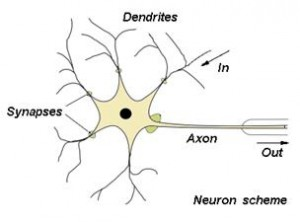
\includegraphics[width=4cm]{figures/1174087/6/1.png}
		\centering
		\caption{Contoh Pembobotan Neural Network}
	\end{figure}

	\item Jelaskan konsep pembobotan dalam neural network. dilengkapi dengan ilustrasi atau gambar
	\hfill\break
	Bobot mewakili kekuatan koneksi antar unit. Jika bobot dari node 1 ke node 2 memiliki besaran lebih besar, itu berarti bahwa neuron 1 memiliki pengaruh lebih besar terhadap neuron. 2. Bobot penting untuk nilai input. Bobot mendekati nol berarti mengubah input ini tidak akan mengubah output. Bobot negatif berarti meningkatkan input ini akan mengurangi output. Bobot menentukan seberapa besar pengaruh input terhadap output. Seperti contoh berikut :
	\begin{figure}[H]
		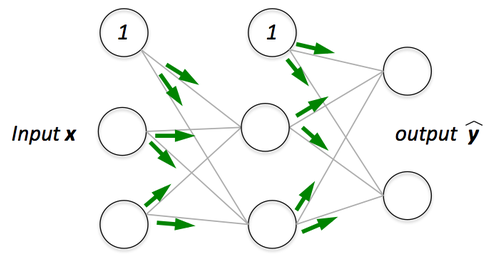
\includegraphics[width=4cm]{figures/1174087/6/2.png}
		\centering
		\caption{Contoh Pembobotan Neural Network}
	\end{figure}

	\item Jelaskan konsep fungsi aktifasi dalam neural network. dilengkapi dengan ilustrasi atau gambar
	\hfill\break
	Fungsi aktivasi digunakan untuk memperkenalkan non-linearitas ke jaringan saraf. Ini menekan nilai dalam rentang yang lebih kecil yaitu. fungsi aktivasi Sigmoid memeras nilai antara rentang 0 hingga 1. Ada banyak fungsi aktivasi yang digunakan dalam industri pembelajaran yang dalam dan ReLU, SeLU dan TanH lebih disukai daripada fungsi aktivasi sigmoid. Ilustrasinya, ketika fungsi aktivasi linier, jaringan saraf dua lapis mampu mendekati hampir semua fungsi. Namun, jika fungsi aktivasi identik dengan fungsi aktivasi F (X) = X), properti ini tidak puas, dan jika MLP menggunakan fungsi aktivasi yang sama, seluruh jaringan setara dengan jaringan saraf lapis tunggal.

	\item Jelaskan cara membaca hasil plot dari MFCC,dilengkapi dengan ilustrasi atau gambar
	\hfill\break
	Berikut merupakan hasil plot dari rekaman suara :
	\begin{figure}[H]
		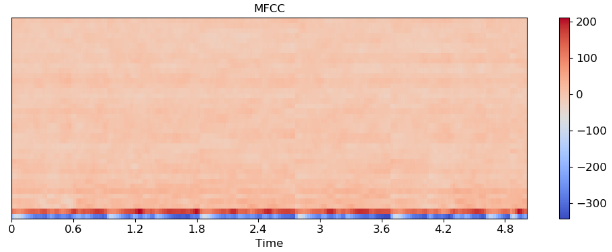
\includegraphics[width=4cm]{figures/1174087/6/3.png}
		\centering
		\caption{Cara Membaca Hasil Plot MFCC}
	\end{figure}
	Dari gambar tersebut dapat diketahui :
	\begin{itemize}
		\item Terdapat 2 dimensi yaitu x sebagai waktu, dan y sebagai power atau desibel.
		\item Dapat dilihat bahwa jika berwarna biru maka power dari suara tersebut rendah, dan jika merah power dari suara tersebut tinggi
		\item Dibagian atas terdapat warna merah pudar yang menandakan bahwa tidak ada suara sama sekali dalam jangkauan tersebut.
	\end{itemize}
	
	\item Jelaskan apa itu one-hot encoding,dilengkapi dengan ilustrasi kode dan atau gambar.
	\hfill\break
	One-hot encoding adalah representasi variabel kategorikal sebagai vektor biner. Mengharuskan nilai kategorikal dipetakan ke nilai integer. Kemudian, setiap nilai integer direpresentasikan sebagai vektor biner yang semuanya bernilai nol kecuali indeks integer, yang ditandai dengan 1.
	\begin{figure}[H]
		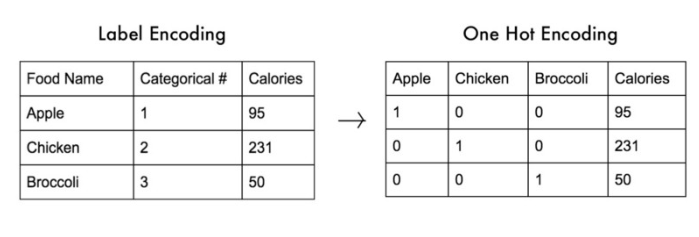
\includegraphics[width=4cm]{figures/1174087/6/4.png}
		\centering
		\caption{One Hot Encoding}
	\end{figure}

	\item Jelaskan apa fungsi dari np/.unique dan to categorical dalam kode program,dilengkapi dengan ilustrasi atau gambar.
	\hfill\break
	Untuk np unique fungsinya yaitu menemukan elemen unik array. Mengembalikan elemen unik array yang diurutkan. Ada tiga output opsional selain elemen unik:\\
	\begin{itemize}
		\item Indeks array input yang memberikan nilai unik
		\item Indeks array unik yang merekonstruksi array input
		\item Berapa kali setiap nilai unik muncul dalam array input.
	\end{itemize}
	\begin{figure}[H]
		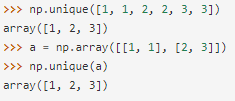
\includegraphics[width=4cm]{figures/1174087/6/5.png}
		\centering
		\caption{Numpy Unique}
	\end{figure}

	Untuk  To Categorical fungsinya untuk mengubah vektor kelas (integer) ke matriks kelas biner.
	\begin{figure}[H]
		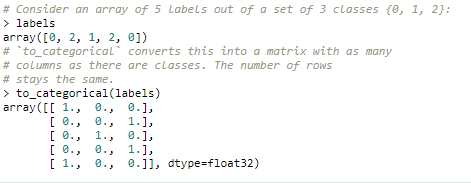
\includegraphics[width=4cm]{figures/1174087/6/6.png}
		\centering
		\caption{To Categorical}
	\end{figure}

	\item Jelaskan apa fungsi dari Sequential dalam kode program,dilengkapi dengan ilustrasi atau gambar.
	\hfill\break
	Sequential berfungsi sebagai tumpukan linear lapisan. COntohnya sebagai berikut :
	\begin{figure}[H]
		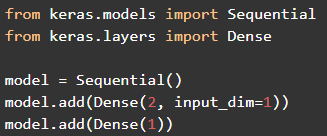
\includegraphics[width=4cm]{figures/1174087/6/7.png}
		\centering
		\caption{Sequential}
	\end{figure}

\end{enumerate}

\subsection{Praktek Program}
\begin{enumerate}
	\item Soal 1
	\hfill\break
	\lstinputlisting[firstline=7, lastline=28]{src/1174087/6/1174087.py}
	Kode di atas menjelaskan cara mengimport library yang dibutuhkan dan membuat fungsi display mfcc untuk melakukan plot pada file audio nanti. Isi data GTZAN adalah datasets lagu atau suara yang terdiri dari 10 gendre yang di simpan kedalam 10 folder yaitu folder blues, classical, country, disco, hiphop, jazz, metal, pop, reggae, dan rock ke sepuluh folder tersebut masing-masing  berisi 100 data suara sedangkan data freesound merupakan contoh data suara yang akan di gunakan untuk menguji hasil pengolahan data tersebut dengan menggunakan metode mfcc. jika GTZAN memiliki beberapa genre jika freesound hanya untuk 1 lagu dan disini kita membuat fungsi untuk membaca file audio dan outputnya sebagai plot, hasilnya adalah sebagai berikut:
	\begin{figure}[H]
	\centering
		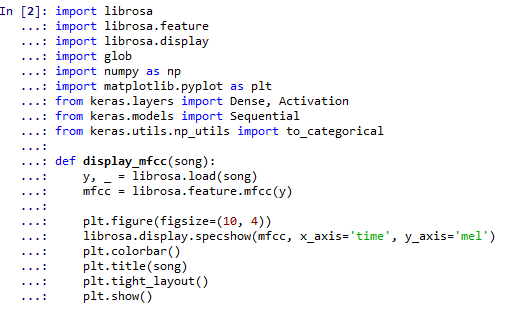
\includegraphics[width=4cm]{figures/1174087/6/8.png}
		\caption{Hasil Soal 1.}
	\end{figure}

	\item Soal 2
	\hfill\break
	\lstinputlisting[firstline=29, lastline=52]{src/1174087/6/1174087.py}
	Kode di atas akan menampilkan hasil dari proses mfcc yang sudah dibuat fungsi pada soal 1, yaitu fungsi display mfcc akan menampilkan plot dari pembacaan file audio. Berikut adalah hasil dari salah satu pembacaan file audio :
	\begin{figure}[H]
	\centering
		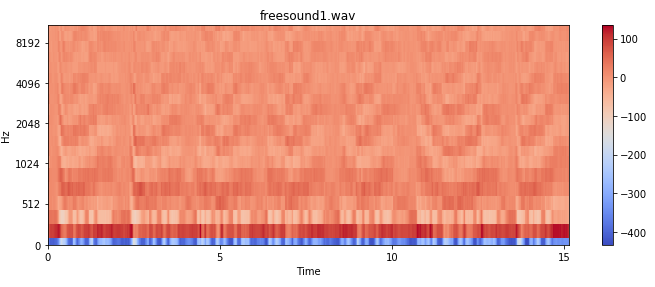
\includegraphics[width=4cm]{figures/1174087/6/9.png}
		\caption{Hasil Soal 2.}
	\end{figure}

	\item Soal 3
	\hfill\break
	\lstinputlisting[firstline=53, lastline=63]{src/1174087/6/1174087.py}
	Kode di atas adalah membuat fungsi yang didefinisikan dengan nama extract\_features\_song yang nantinya akan di gunakan pada fungsi yang lainya kemudian dibuat variabel y dengan method librosa load setelah itu dibuat variabel baru mfcc dengan isi librosa features mfcc dengan isi variabel y tadi kemudian dibuat variabel mfcc dengan isian np.max dan variabel mfcc tadi terakhir di buat array dari data tersebut merupakan data 25000 data pertama. kenapa data 25000 pertama yang digunakan dikarenakan data tersebut digunakan sebagai data testing semakin besar data testing yang di gunakan maka semakin akurat hasil AI. tapi sebenarnya data tersebut relatif bisa lebih besar atau lebih kecil tergantung pada komputer masing masing. Hasilnya adalah sebagai berikut :
	\begin{figure}[H]
	\centering
		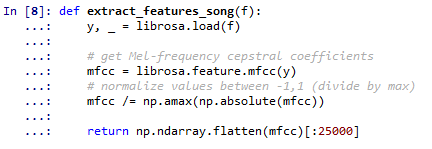
\includegraphics[width=4cm]{figures/1174087/6/10.png}
		\caption{Hasil Soal 3.}
	\end{figure}

	\item Soal 4
	\hfill\break
	\lstinputlisting[firstline=65, lastline=84]{src/1174087/6/1174087.py}
	Kode di atas adalah mendefinisian nama fungsi yaitu generate features and labels kemudian membuat variabel baru dengan array kosing yaitu all\_features dan all\_labels kemudian mendefinisikan isian label untuk gendre dengan cara membuat variabel genres kemudian di isi dengan 10 gendre yang tadi setelah itu dilakukan fungsi if else dengan code for dan in setelah itu akan di buat encoding untuk data tiap tiap label contoh untuk blues 1000000000 dan untuk clasical 0100000000. Hasilnya adalah sebagai berikut :
	\begin{figure}[H]
	\centering
		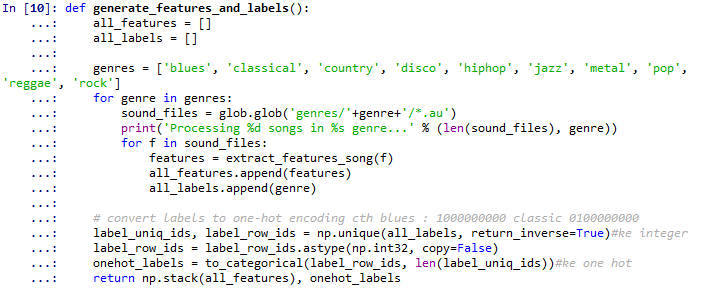
\includegraphics[width=4cm]{figures/1174087/6/11.png}
		\caption{Hasil Soal 4.}
	\end{figure}

	\item Soal 5
	\hfill\break
	\lstinputlisting[firstline=86, lastline=90]{src/1174087/6/1174087.py}
	Hal ini menjadi lama dikarenakan mesin membaca satupersatu file yang ada pada folder dan dalam foldertersebut terdapat 100 file sehingga wajar menjadi lama ditambah lagi mengolah data yang tadinya suara menjadi bentuk vektor. Hasilnya adalah sebagai berikut :
	\begin{figure}[H]
	\centering
		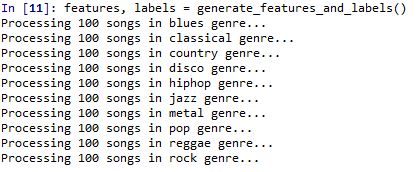
\includegraphics[width=4cm]{figures/1174087/6/12.png}
		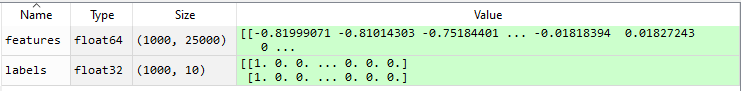
\includegraphics[width=4cm]{figures/1174087/6/13.png}
		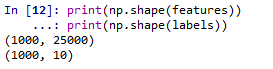
\includegraphics[width=4cm]{figures/1174087/6/14.png}
		\caption{Hasil Soal 5.}
	\end{figure}

	\item Soal 6
	\hfill\break
	\lstinputlisting[firstline=91, lastline=110]{src/1174087/6/1174087.py}
	Kode diatas berfungsi untuk melakukan training split 80\%. Karena supaya mesin dapat terus belajar tentang data baru, jadi ketika prediksi dibuat tentang data yang terlatih itu bisa mendapatkan persentase yang cukup bagus. Hasilnya adalah sebagai berikut :
	\begin{figure}[H]
	\centering
		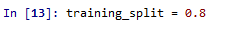
\includegraphics[width=4cm]{figures/1174087/6/15.png}
		\caption{Hasil Soal 6.}
	\end{figure}

	\item Soal 7
	\hfill\break
	\lstinputlisting[firstline=112, lastline=118]{src/1174087/6/1174087.py}
	Fungsi Sequential() ialah Sebuah model untuk menentukan izin pada setiap neuron, di sini adalah 100 dense yang merupakan 100 neuron pertama dari data pelatihan. Fungsi dari relay itu sendiri adalah untuk mengaktifkan neuron atau input yang memiliki nilai maksimum. Sedangkan untuk dense 10 itu adalah output dari hasil neuron yang telah berhasil diaktifkan, untuk dense 10 diaktifkan menggunakan softmax. Hasilnya adalah sebagai berikut :
	\begin{figure}[H]
	\centering
		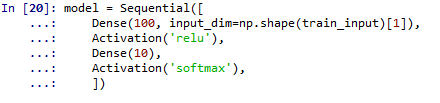
\includegraphics[width=4cm]{figures/1174087/6/16.png}
		\caption{Hasil Soal 7.}
	\end{figure}

	\item Soal 8
	\hfill\break
	\lstinputlisting[firstline=119, lastline=123]{src/1174087/6/1174087.py}
	Model Compile di perjelas dengan gambar dibawah, Hasil output pada kode tersebut seperti gambar  menjelaskan bahwa dense pertama itu memiliki 100 neurons dengan parameter sekitar 2 juta lebih dengan aktviasi 100, jadi untuk setiap neurons memiliki masing-masing 1 aktivasi. Sama halnya seperti dense 2 memiliki jumlah neurons sebanyak 10 dengan parameter 1010 dan jumlah aktivasinya 10 untuk setiap neurons tersebut dan total parameternya sekitar 2.5 juta data yang akan dilatih pada mesin tersebut.
	\begin{figure}[H]
	\centering
		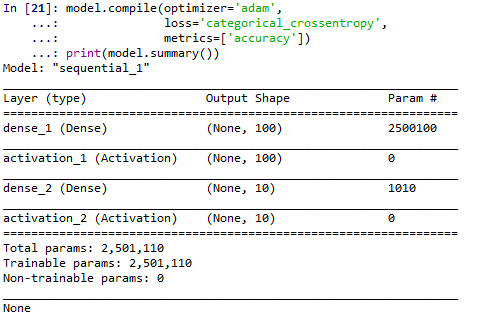
\includegraphics[width=4cm]{figures/1174087/6/17.png}
		\caption{Hasil Soal 8.}
	\end{figure}

	\item Soal 9
	\hfill\break
	\lstinputlisting[firstline=124, lastline=126]{src/1174087/6/1174087.py}
	Kode tersebut berfungsi untuk melatih mesin dengan data training input dan training label. Epochs ini merupakan iterasi atau pengulangan berapa kali data tersebut akan dilakukan. Batch\_size ini adalah jumlah file yang akan dilakukan pelatihan pada setiap 1 kali pengulangan. Sedangkan validation\_split itu untuk menentukan presentase dari cross validation atau k-fold sebanyak 20\% dari masing-masing data pengulangan, hasilnya adalah sebagai berikut :
	\begin{figure}[H]
	\centering
		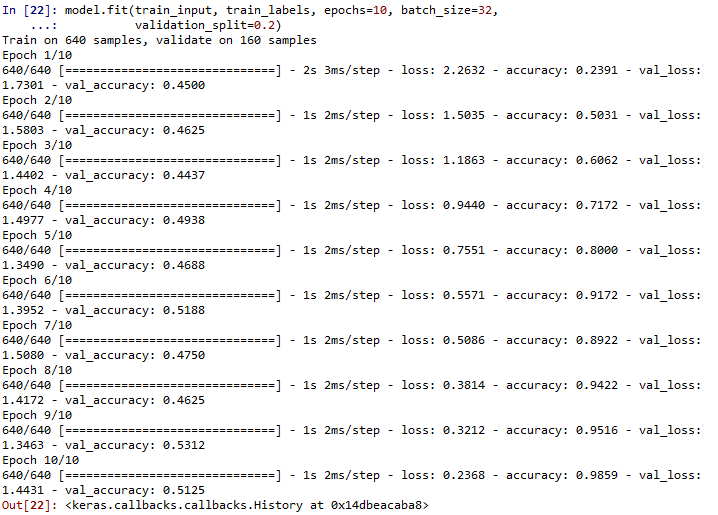
\includegraphics[width=4cm]{figures/1174087/6/18.png}
		\caption{Hasil Soal 9.}
	\end{figure}

	\item Soal 10
	\hfill\break
	\lstinputlisting[firstline=127, lastline=131]{src/1174087/6/1174087.py}
	Fungsi evaluate atau evaluasi ini ialah untuk menguji data pengujian setiap file. Di sini ada prediksi yang hilang, artinya mesin memprediksi data, sedangkan untuk keseluruhan perjanjian sekitar 55\%, hasilnya adalah sebagai berikut :
	\begin{figure}[H]
	\centering
		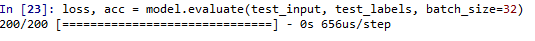
\includegraphics[width=4cm]{figures/1174087/6/19.png}
		\caption{Hasil Soal 10.}
	\end{figure}

	\item Soal 11
	\hfill\break
	\lstinputlisting[firstline=133, lastline=134]{src/1174087/6/1174087.py}
	Fungsi Predict ialah untuk menghasilkan suatu nilai yang sudah di prediksi dari data training sebelumnya. Gambar dibawah ini menjelaskan file yang di jalankan tersebut termasuk ke dalam genre apa, hasilnya bisa dilihat pada gambar tersebut presentase yang paling besar yakni genre rock. Maka lagu tersebut termasuk ke dalam genre rock dengan perbandingan presentase hasil prediksi.
	\begin{figure}[H]
	\centering
		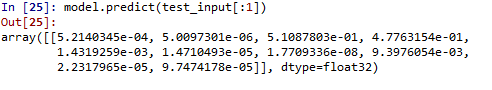
\includegraphics[width=4cm]{figures/1174087/6/20.png}
		\caption{Hasil Soal 11.}
	\end{figure}
\end{enumerate}

\subsection{Penanganan Error}
\begin{enumerate}
	\item ScreenShoot Error
	\begin{figure}[H]
		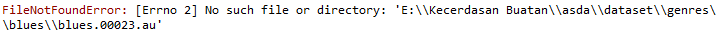
\includegraphics[width=4cm]{figures/1174087/6/error.png}
		\centering
		\caption{FileNotFoundError}
	\end{figure}

	\item Cara Penanganan Error
	\begin{itemize}
		\item FileNotFoundError
		\hfill\break
		Error terdapat pada letak file yang tidak terbaca, karena letak file berbeda dengan pemanggilannya, solusi nya ialah dengan meletakkan direktori file yang dibaca dengan benar.
	\end{itemize}
\end{enumerate}

\subsection{Bukti Tidak Plagiat}
\begin{figure}[H]
\centering
	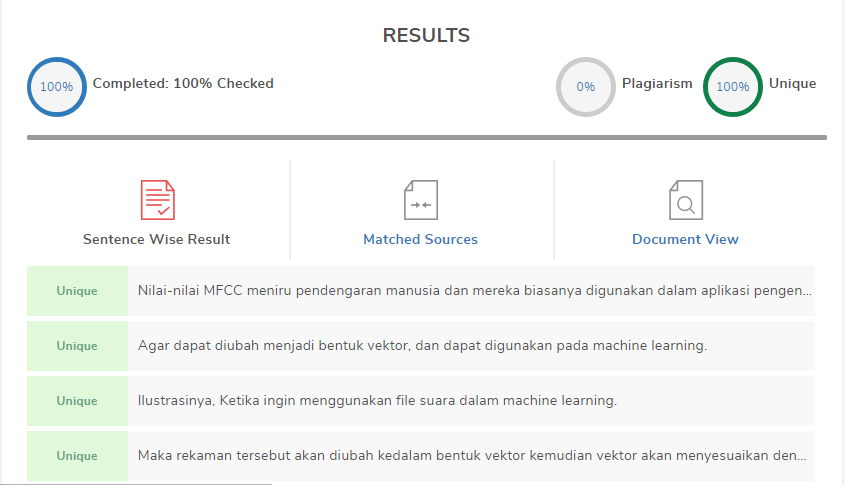
\includegraphics[width=4cm]{figures/1174087/6/plagiat.png}
	\caption{Bukti Tidak Melakukan Plagiat Chapter 6}
\end{figure}